% ---- pg-043 （书页 31） ----

$(D,2))+d((D,2),(C,2))=1+1=2$, 或是 $d((D,1),(C,2))=d((D,1),(C,1))+d((C,1),%
(C,2))=1+1=2$. )

\begin{mvfigure}
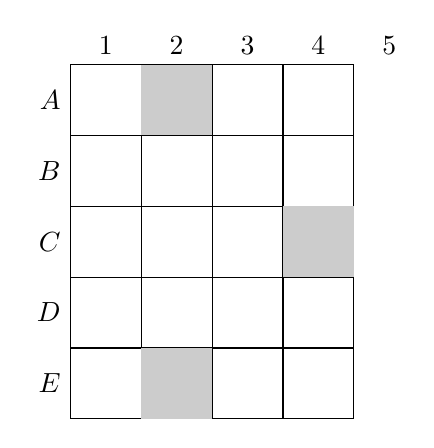
\begin{tikzpicture}[scale=0.9]
\draw[step=1cm] (0,0) grid (4,5);
\fill[gray!40] (1,4) rectangle (2,5);
\fill[gray!40] (3,2) rectangle (4,3);
\fill[gray!40] (1,0) rectangle (2,1);
\foreach \y/\l in {4.5/A,3.5/B,2.5/C,1.5/D,0.5/E} \node[left] at (0,\y) {$\l$};
\foreach \x/\n in {0.5/1,1.5/2,2.5/3,3.5/4,4.5/5} \node[above] at (\x,5) {\n};
\end{tikzpicture}
\end{mvfigure}

在一个交点上设置一个供应机构(仓库), 使得从仓库到 3 个零售商店的距离总和最小. 以下的练习包含相当大的数据集, 或许需要一台计算机来完成所需的计算.

\mvbold{1.14} \hyperref[tab:1.6]{表 1.6} 包含一些在 1.2 节中讨论过的未处理的数据 (参见网页 www. prenhall. com/statistics 上的多发性硬化症数据), 两种不同的视觉刺激 (S1 和 S2) 对研究人群中实验对象的左眼(L)和右眼(R)都产生影响. 表中记录的值包括 $x_1$(参加实验者的年龄); $x_2$(刺激 S1 对两眼总影响, 即 $\mathrm{S1L}+\mathrm{S1R}$); $x_3$(刺激 S1 对两眼影响之差, 即 $|\mathrm{S1L}-\mathrm{S1R}|$); 如此类推.

\begin{mvtable}
\phantomsection\label{tab:1.6}\mvtabcap{表 1.6\quad 多发性硬化症数据}
\begin{tabular}{ccccc}
\toprule
\multicolumn{5}{c}{非多发性硬化症人群数据} \\
\midrule
实验对象 & $x_1$ & $x_2$ & $x_3$ & $x_4$ \\
序号 & (年龄) & $(\mathrm{S1L}+\mathrm{S1R})$ & $(\mathrm{S1L}-\mathrm{S1R})$ & $(\mathrm{S2L}+\mathrm{S2R})$ \\
\midrule
1 & 18 & 152.0 & 1.6 & 198.4 \\
2 & 19 & 138.0 & 0.4 & 180.8 \\
3 & 20 & 144.0 & 0.0 & 186.4 \\
4 & 20 & 143.6 & 3.2 & 194.8 \\
5 & 20 & 148.8 & 0.0 & 217.6 \\
$\vdots$ & $\vdots$ & $\vdots$ & $\vdots$ & $\vdots$ \\
65 & 67 & 154.4 & 2.4 & 205.2 \\
66 & 69 & 171.2 & 1.6 & 210.4 \\
67 & 73 & 157.2 & 0.4 & 204.8 \\
68 & 74 & 175.2 & 5.6 & 235.6 \\
69 & 79 & 155.0 & 1.4 & 204.4 \\
\midrule
\multicolumn{5}{c}{多发性硬化症人群数据} \\
\midrule
实验对象 & $x_1$ & $x_2$ & $x_3$ & $x_4$ \\
序号 &  &  &  &  \\
\midrule
1 & 23 & 148.0 & 0.8 & 205.4 \\
2 & 25 & 195.2 & 3.2 & 262.8 \\
3 & 25 & 158.0 & 8.0 & 209.8 \\
4 & 28 & 134.4 & 0.0 & 198.4 \\
5 & 29 & 190.2 & 14.2 & 243.8 \\
$\vdots$ & $\vdots$ & $\vdots$ & $\vdots$ & $\vdots$ \\
25 & 57 & 165.6 & 16.8 & 229.2 \\
26 & 58 & 238.4 & 8.0 & 304.4 \\
27 & 58 & 164.0 & 0.8 & 216.8 \\
28 & 58 & 169.8 & 0.0 & 219.2 \\
29 & 59 & 199.8 & 4.6 & 250.2 \\
\bottomrule
\end{tabular}
\end{mvtable}

{\zihao{6} 资料来源：数据经 G. G. Celeisa 博士许可使用.}

% UNCERTAIN: pg-043 \hyperref[tab:1.6]{表 1.6} 表头第五列 $x_5$ 及其下方 $(\mathrm{S2L}-\mathrm{S2R})$ 的列位置按原书排在其右侧,本转写合并为一个五列表; 数据行末第五列值(如 0.0,1.6,…)原书印在 $x_5$ 列,此处未单列(原页右侧边缘截断)
